%\documentclass[a4paper,12pt]{book}
%\usepackage{pgfplots}
%\usepackage[justification=centering]{caption}
%\pgfplotsset{compat=newest}
%\begin{document}
\chapter{Experimental Result}
In this chapter we have shown our experimental results achieved by our proposed approach. Based on several performance metric we have tried to show our algorithms' efficiency and performance. We have taken different scale/parameter to evaluate our algorithm
\section{Experimental Settings}
We have performed number of simulations in our experiment on both synthetic database and real world database. The data are taken from data set repository [\ref{bib:dataset}]. Our experiment shows that \emph{US-tree} ( Uncertain Stream tree )is very much compact. This tree construction technique can make the items to share one node. This compactness of \emph{US-tree} surprisingly helps the mining, \emph{USFP-growth} ( Uncertain Stream Frequent Pattern growth ) process to gain a lot in run-time and memory. More over our proposed pattern tree can be used to find max patterns and close patterns. Performance tests from our experiment shows that \emph{US-tree} tree construction technique and \emph{USFP-growth} mining algorithm can run on any uncertain stream database with any support threshold, window size and batch size. Our experimental result shows that these techniques are much more faster and scalable frequent pattern mining technique. As we have proposed a new approach for finding frequent patterns over uncertain data we have compared performance with itself for comparing correctness of our approach. Then we have compared with all well known existing approaches for finding frequent item sets over uncertain database. \emph{SUF-growth} is one of them. We have tried to compare in all aspects to prove our approach's correctness, run-time efficiency, memory efficiency and and scalability.
%\documentclass{article} 
%
%\begin{document}
\begin{table}
\centering

\begin{tabular}{|l|l|}
\hline 
	Property&Configurations\\ \hline\hline

	Processor				& Intel(R) Core(TM) i7		\\ \hline
	Core Count				& 8							\\\hline
	Memory					& 8 GB RAM 					\\\hline
	OS Name					& Windows					\\ \hline
	OS version 				& 7, service pack 1 		\\ \hline
	OS Architecture 		& 64 bit					\\ \hline
	Programming Language 	& Java						\\ \hline
	Development Kit 		& JDK						\\ \hline
	Development Kit Version & 1.7 SE.					\\\hline
	Virtual Machine 		& JVM						\\ \hline
	Runtime Environment 	& JRE 7						\\\hline
	Build Tool				& Gradle					\\\hline
	Build Tool Version		& 2.6						\\\hline
	\end{tabular}
\caption{Configuration of Experimental Environment}
\label{table:experiment_configuration}
\end{table}
%\end{document}
All program for the simulating experimental result are written \emph{Java} programming language that run on \emph{Java Runtiime Environment (JRE) - 1.7.0.79}. All program was run on a computer having \emph{3.4GHz Intel(R) Core(TM) i7} processor and \emph{8GB RAM} with \emph{Windows-7, 64-bit, service pack-1} operating system installed in it (Table-[\ref{table:experiment_configuration}]). Results shown in this chapter are based on average of multiple run for every case. \emph{US-tree} was constructed with chronological order of database items. All the running time includes \emph{CPU}, \emph{I/O}.\\
\documentclass{article}
\usepackage{pgfplots}
\begin{document}
\pgfmathdeclarefunction{gauss}{2}{%
  \pgfmathparse{1/(#2*sqrt(2*pi))*exp(-((x-#1)^2)/(2*#2^2))}%
}
\begin{figure}
\centering
\begin{tikzpicture}
\begin{axis}[
 width=11cm,
   height=8cm,
  no markers, domain=0:1, samples=1000,
  axis lines*=left, xlabel=Items, ylabel=Uncertaininty Value,
%  every axis y label/.style={at=(current axis.above origin),anchor=south},
  every axis x label/.style={at=(current axis.right of origin),anchor=west},
  height=5cm, width=12cm,
  xtick={.5}, ytick=\empty,
  enlargelimits=false, clip=false, axis on top,
  grid = major
  ]

  \addplot [thick,cyan!50!blue] {gauss(.5,.159154943)};
\end{axis}

\end{tikzpicture}
\caption{Normal Distribution}
\label{result:normal_distribution}
\end{figure}
\end{document}
we got the synthetic and real life datasets from the frequent itemset mining repository [\ref{bib:dataset}], those were collected for certain databases. Then we have used our own probabilistic tool and technique to generate existential probability of each items of the each transaction of database. Real life data set actually follows gaussian distribution that is normal distribution [\ref{result:normal_distribution}]. It actually says that in real world extreme cases are minimum and average case are maximum. From the figure [\ref{result:normal_distribution}] we can see that in the middle the pick value is highest so we can say count item probability at \emph{.5} is maximum. So we used this technique to generate and introduce existential probability to each items in a transaction. We have used \emph{Java psudo random} generate existential probability for each item of all the transaction of database. By assigning these probabiity value to each items we have generate uncertain database for both real life database and synthetic database found from dataset repository [\ref{bib:dataset}]. However one can give existential probability by any distribution according to need.
\section{Performance Metrics}
We have consider several metrics as parameters for evaluating our proposed algorithm. We have set several property for this evaluation from experimental result. As we have worked on data set that comes like stream so we have set parameters for both the frequent item set mining from total data set and per window. The parameters and properties are given below:

\begin{itemize}
\item Tree construction time per window and total database vs minimum support.
\item Mining time per window and total database vs minimum support.
\item Total time to complete per window and total database vs minimum support.
\item Total tree node in tree per window.
\item Total memory needed by mining process
\end{itemize}
\section{Experimental Environment}
For our experimental evaluation we used both real life database and synthetic database from database repository [\ref{bib:dataset}]. Table [\ref{table:dataset}] shows the data base type and properties.
\begin{table}[t]
\centering
\begin{tabular}{|l|l|l|l|l|}
\hline 
\textbf{Name}&\textbf{Type}&\textbf{Density}&\textbf{Total Transaction} &\textbf{Distinct Items}\\ \hline
mushroom	&	real	&	dense	&	8124	&	120\\ \hline
kosarak	&	real	&	sparse	&	990002	&	41270\\ \hline
pumsb star	&	real	&	sparse	&	49046	&	2088\\ \hline
chess	&	real	&	dense	&	3196	&	75\\ \hline
T10I4D100K	&	synthetic	&	sparse	&	100000	&	869\\ \hline
	\end{tabular}
\caption{Dataset from repository [\ref{bib:dataset}]}
\label{table:dataset}
\end{table}
\subsection{Real Life Data Set}
For real life data sets we have used mushroom [\ref{bib:dataset}], chess [\ref{bib:dataset}] and pumsb star [\ref{bib:dataset}]. Mushroom, chess and pumsb star are dense datasets. Mushroom has 8124 transactions with 120 distinct items, chess has 3196 transactions with 75 distinct items and pumsb star has 49046 transactions with 2088 distinct items. For probability assignment to each items we used normal distribution for getting existential probability.
\subsection{Synthetic Data Set}
For synthetic data sets we have used T10I4D100K [\ref{bib:dataset}]. It is an IBM generated transactional data set widely used for frequent pattern mining. It is a sparse data set with 100000 transactions and 869 distinct items. For probability assignment to each items we used normal distribution for getting existential probability.
%%mark = star, diamond, square, otimes
%\documentclass{article}
%\usepackage{pgfplots}
%\usepackage[justification=centering]{caption}
%\pgfplotsset{compat=newest}
%\begin{document}
\begin{figure}
\centering

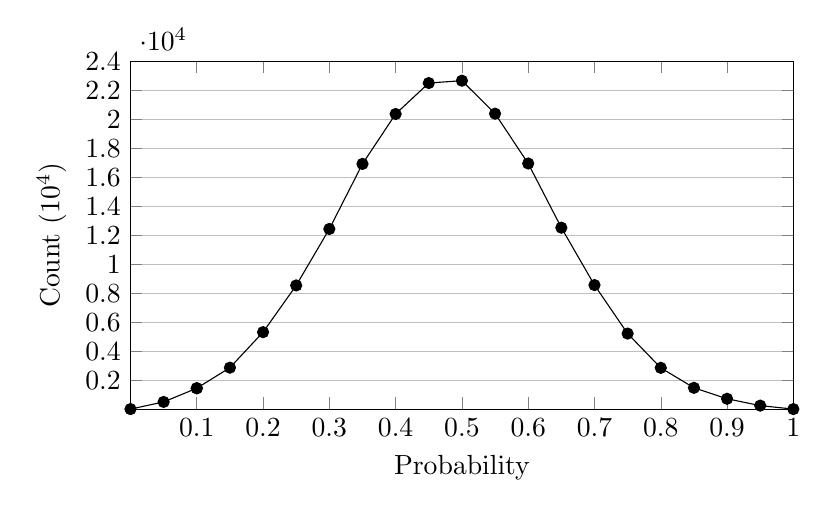
\begin{tikzpicture}
\begin{axis}[
 width=10cm,
   height=6cm,
    xlabel={Probability },
    ylabel={Count ($10^4$)},
    xmin=0, xmax=1.0,
    ymin=0, ymax=24000,
    xtick={.1,.2,.3,.4,.5,.6,.7,.8,.9,1.0},
    ytick={2000,4000,6000,8000,10000,12000,14000,16000,18000,20000,22000,24000},
    legend pos=north east,
    ymajorgrids=true,
    grid style={line width=.2pt,draw=gray!50},
]
 
\addplot[
    solid, every mark/.append style={solid, fill=black}, mark=*
    ]
    coordinates {
		(0,0)
		(.05,495)
		(0.1,1439)
		(0.1 ,1439)
		(0.15,2859)
		(0.2 ,5307)
		(0.25,8531)
		(0.3 ,12426)
		(0.35,16915)
		(0.4 ,20358)
		(0.45,22493)
		(0.5 ,22655)
		(0.55,20380)
		(0.6 ,16943)
		(0.65,12514)
		(0.7 ,8555)
		(0.75,5209)
		(0.8 ,2845)
		(0.85,1468)
		(0.9 ,712)
		(0.95,240)
		(1.0,0)
};
 
\end{axis}
\end{tikzpicture}
%\caption{Probability Distribution for \emph{Mushroom} data set}
\label{result:data_mushroom}
\end{figure}
%\end{document}
%%mark = star, diamond, square, otimes
%\documentclass{article}
%\usepackage{pgfplots}
%\usepackage[justification=centering]{caption}
%\pgfplotsset{compat=newest}
%\begin{document}
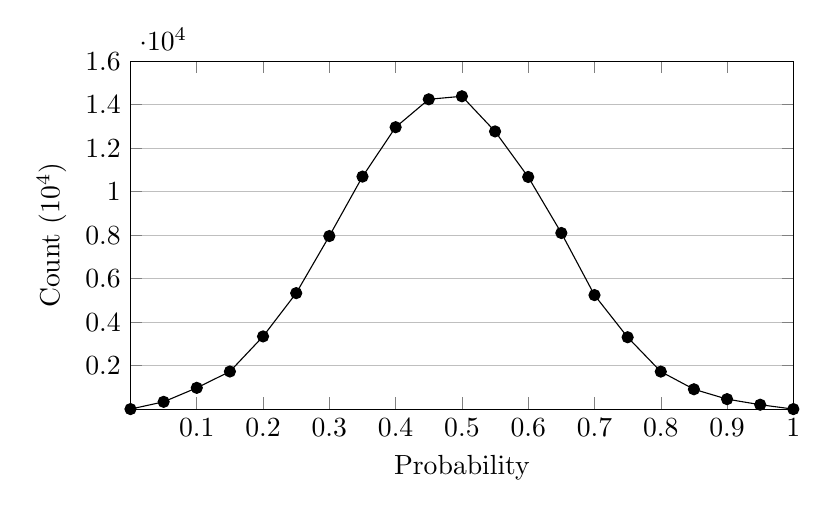
\begin{tikzpicture}
\begin{axis}[
 width=10cm,
   height=6cm,
    xlabel={Probability },
    ylabel={Count ($10^4$)},
    xmin=0, xmax=1.0,
    ymin=0, ymax=16000,
    xtick={.1,.2,.3,.4,.5,.6,.7,.8,.9,1.0},
    ytick={2000,4000,6000,8000,10000,12000,14000,16000},
    legend pos=north east,
    ymajorgrids=true,
    grid style={line width=.2pt,draw=gray!50},
]
 
\addplot[
    solid, every mark/.append style={solid, fill=black}, mark=*
    ]
    coordinates {
			(0,0)
			(0.05,334)
			(0.1,977)
			(0.15,1729)
			(0.2,3342)
			(0.25,5333)
			(0.3,7958)
			(0.35,10692)
			(0.4,12964)
			(0.45,14247)
			(0.5,14386)
			(0.55,12770)
			(0.6,10675)
			(0.65,8099)
			(0.7,5242)
			(0.75,3304)
			(0.8,1724)
			(0.85,912)
			(0.9,458)
			(0.95,201)
			(1,0)

};
 
\end{axis}
\end{tikzpicture}
%\end{document}
%%mark = star, diamond, square, otimes
%\documentclass{article}
%\usepackage{pgfplots}
%\usepackage[justification=centering]{caption}
%\pgfplotsset{compat=newest}
%\begin{document}
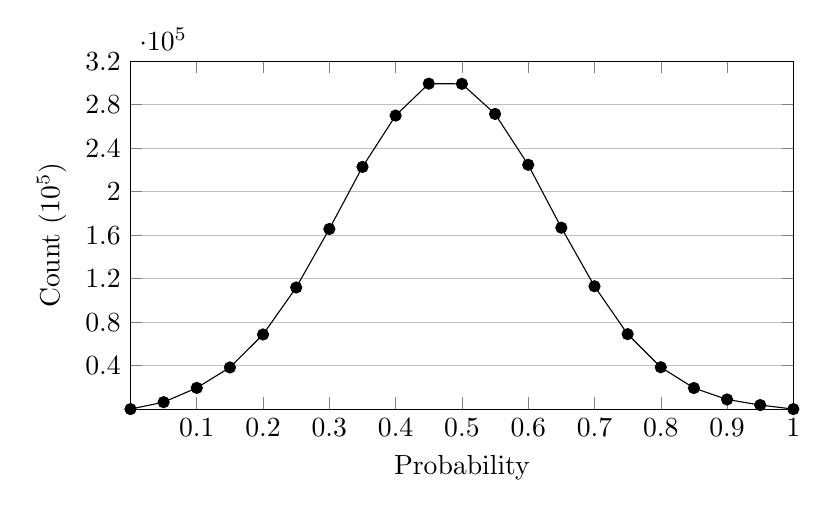
\begin{tikzpicture}
\begin{axis}[
 width=10cm,
   height=6cm,
    xlabel={Probability },
    ylabel={Count ($10^5$)},
    xmin=0, xmax=1.0,
    ymin=0, ymax=320000,
    xtick={.1,.2,.3,.4,.5,.6,.7,.8,.9,1.0},
    ytick={40000,80000,120000,160000,200000,240000,280000,320000},
    legend pos=north east,
    ymajorgrids=true,
    grid style={line width=.2pt,draw=gray!50},
]
 
\addplot[
    solid, every mark/.append style={solid, fill=black}, mark=*
    ]
    coordinates {
			(0,0)
			(0.05,6362)
			(0.1,19508)
			(0.15,38310)
			(0.2,68623)
			(0.25,111854)
			(0.3,165662)
			(0.35,222758)
			(0.4,269985)
			(0.45,299328)
			(0.5,299159)
			(0.55,271454)
			(0.6,224689)
			(0.65,166840)
			(0.7,112959)
			(0.75,68933)
			(0.8,38490)
			(0.85,19368)
			(0.9,8848)
			(0.95,3707)
			(1,0)
};
 
\end{axis}
\end{tikzpicture}
%\end{document}
%mark = star, diamond, square, otimes
%\documentclass{article}
%\usepackage{pgfplots}
%\usepackage[justification=centering]{caption}
%\pgfplotsset{compat=newest}
%\begin{document}
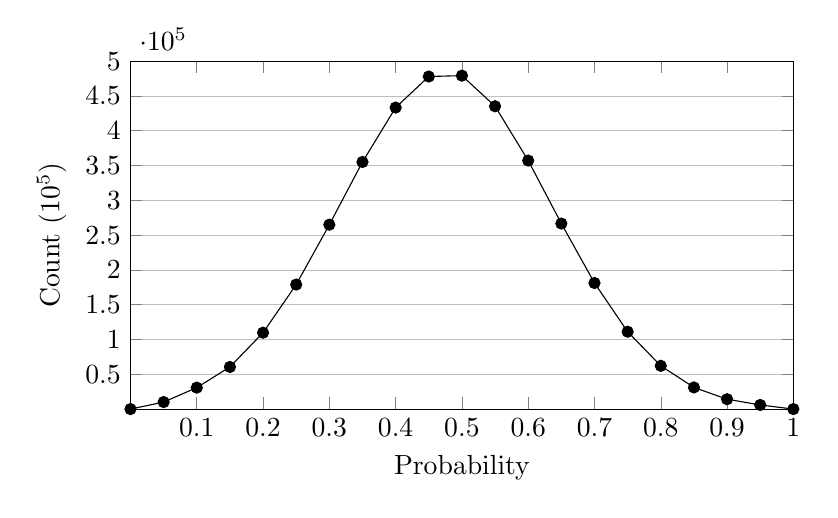
\begin{tikzpicture}
\begin{axis}[
 width=10cm,
   height=6cm,
    xlabel={Probability },
    ylabel={Count ($10^5$)},
    xmin=0, xmax=1.0,
    ymin=0, ymax=500000,
    xtick={.1,.2,.3,.4,.5,.6,.7,.8,.9,1.0},
    ytick={50000,100000,150000,200000,250000,300000,350000,400000,450000,500000},
    legend pos=north east,
    ymajorgrids=true,
    grid style={line width=.2pt,draw=gray!50},
]
 
\addplot[
    solid, every mark/.append style={solid, fill=black}, mark=*
    ]
    coordinates {
			(0,0)
			(0.05,10068)
			(0.1,30825)
			(0.15,60529)
			(0.2,109792)
			(0.25,178975)
			(0.3,265006)
			(0.35,355127)
			(0.4,433334)
			(0.45,477961)
			(0.5,479225)
			(0.55,435233)
			(0.6,357179)
			(0.65,266639)
			(0.7,181169)
			(0.75,111182)
			(0.8,62178)
			(0.85,31116)
			(0.9,14207)
			(0.95,5909)
			(1,0)
};
 
\end{axis}
\end{tikzpicture}
%\end{document}
\section{Comparison with Existing Approaches}
\subsection{Runtime Comparison}
%%mark = star, diamond, square, otimes
%\documentclass{article}
%\usepackage{pgfplots}
%\usepackage[justification=centering]{caption}
%\pgfplotsset{compat=newest}
%\begin{document}
\begin{figure}
\centering

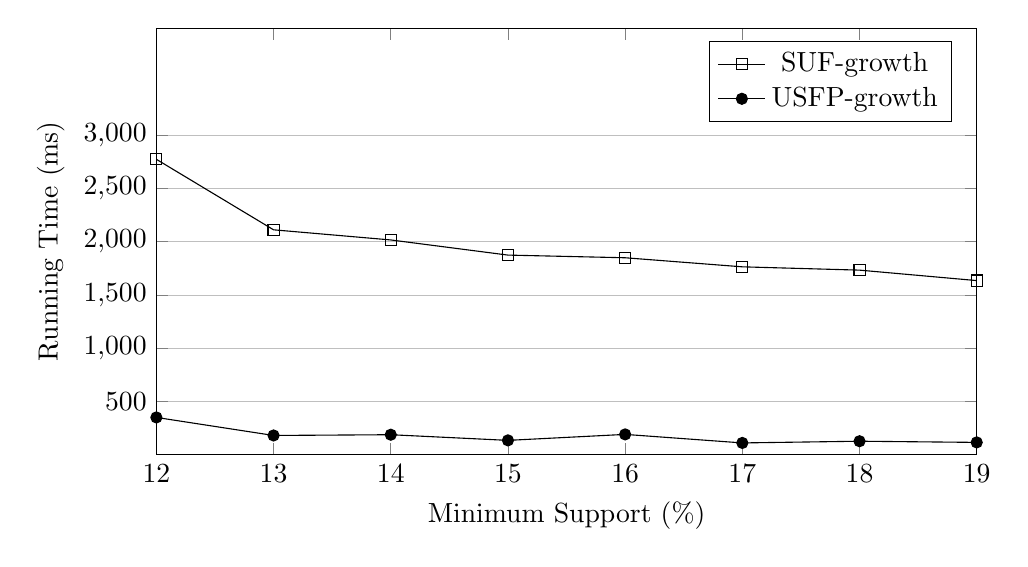
\begin{tikzpicture}
\begin{axis}[
 width=12cm,
   height=7cm,
    xlabel={Minimum Support (\%) },
    ylabel={Running Time (ms)},
    xmin=12, xmax=19,
    ymin=0, ymax=4000,
    xtick={12,13,14,15,16,17,18,19},
    ytick={500,1000,1500,2000,2500,3000},
    legend pos=north east,
    ymajorgrids=true,
    grid style={line width=.2pt,draw=gray!50},
]
 
\addplot[
    solid, every mark/.append style={solid, fill=gray}, mark=square
    ]
    coordinates {
	(12,2771)
	(13,2110)
	(14,2015)
	(15,1873)
	(16,1848)
	(17,1763)
	(18,1732)
	(19,1634)
	};
    \addlegendentry{SUF-growth}
\addplot[
    solid, every mark/.append style={solid, fill=black}, mark=*
    ]
    coordinates {
	(12,351)
	(13,182)
	(14,189)
	(15,136)
	(16,192)
	(17,112)
	(18,128)
	(19,117)
};
    \addlegendentry{USFP-growth}
 
\end{axis}
\end{tikzpicture}
%\caption{Total Tree Construction Time vs Minimum Suppport (\%) \\(Window Size = 4, Frame Size = 650) for mushroom database}
\label{result:mushroom_tree_total}
\end{figure}
%\end{document}
%mark = star, diamond, square, otimes
\documentclass{article}
\usepackage{pgfplots}
\usepackage[justification=centering]{caption}
\pgfplotsset{compat=newest}
\begin{document}
\begin{figure}
\centering

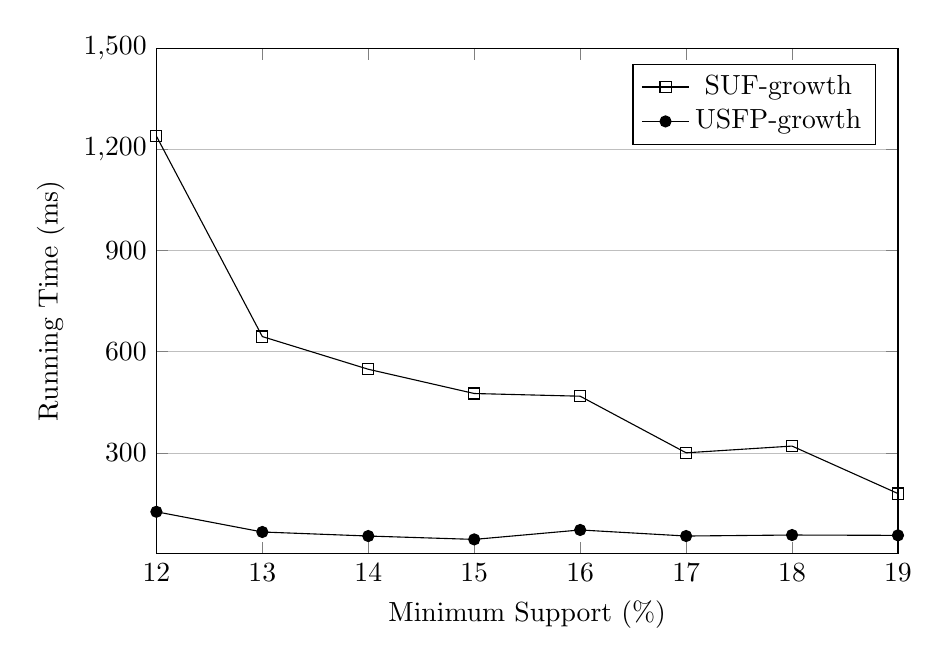
\begin{tikzpicture}
\begin{axis}[
 width=11cm,
   height=8cm,
    xlabel={Minimum Support (\%) },
    ylabel={Running Time (ms)},
    xmin=12, xmax=19,
    ymin=0, ymax=1500,
    xtick={12,13,14,15,16,17,18,19},
    ytick={300,600,900,1200,1500,2000},
    legend pos=north east,
    ymajorgrids=true,
    grid style={line width=.2pt,draw=gray!50},
]
 
\addplot[
    solid, every mark/.append style={solid, fill=gray}, mark=square
    ]
    coordinates {
	(12,1240)
	(13,645)
	(14,548)
	(15,476)
	(16,468)
	(17,300)
	(18,320)
	(19,179)
};
    \addlegendentry{SUF-growth}
\addplot[
    solid, every mark/.append style={solid, fill=black}, mark=*
    ]
    coordinates {
	(12,125)
	(13,65 )
	(14,53 )
	(15,43 )
	(16,71 )
	(17,53 )
	(18,56 )
	(19,55 )
};
    \addlegendentry{USFP-growth}
 
\end{axis}
\end{tikzpicture}
\caption{Total Tree Mining vs Minimum Suppport (\%) \\(Window Size = 4, Frame Size = 650) for mushroom database}
\label{result:mushroom_total}
\end{figure}
\end{document}
%%mark = star, diamond, square, otimes
%\documentclass{article}
%\usepackage{pgfplots}
%\usepackage[justification=centering]{caption}
%\pgfplotsset{compat=newest}
%\begin{document}
\begin{figure}
\centering

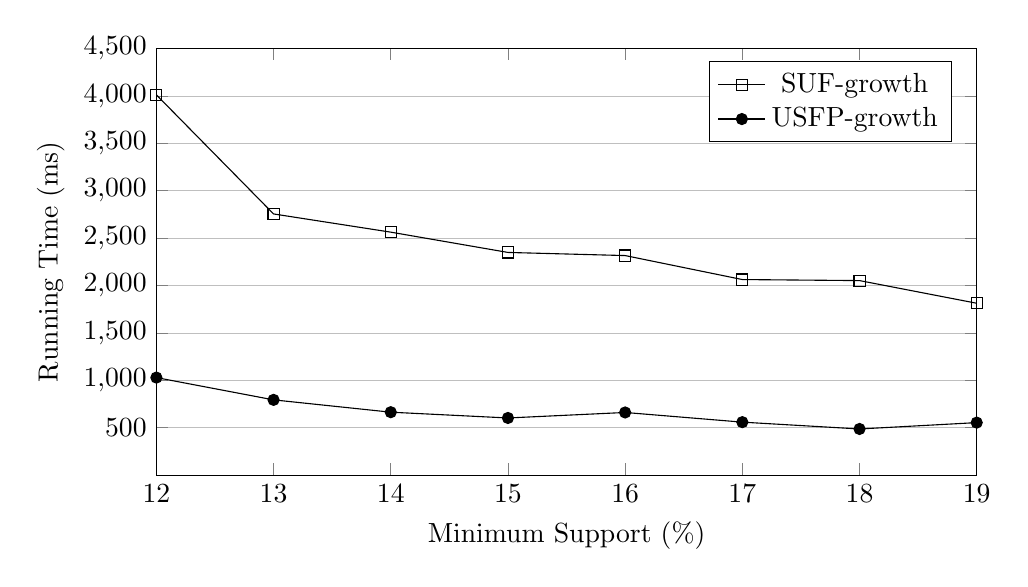
\begin{tikzpicture}
\begin{axis}[
 width=12cm,
   height=7cm,
    xlabel={Minimum Support (\%) },
    ylabel={Running Time (ms)},
    xmin=12, xmax=19,
    ymin=0, ymax=4500,
    xtick={12,13,14,15,16,17,18,19},
    ytick={500,1000,1500,2000,2500,3000,3500,4000,4500},
    legend pos=north east,
    ymajorgrids=true,
    grid style={line width=.2pt,draw=gray!50},
]
 
\addplot[
    solid, every mark/.append style={solid, fill=gray}, mark=square
    ]
    coordinates {
	(12,4011)
	(13,2755)
	(14,2563)
	(15,2349)
	(16,2316)
	(17,2063)
	(18,2052)
	(19,1813)
};
    \addlegendentry{SUF-growth}
\addplot[
    solid, every mark/.append style={solid, fill=black}, mark=*
    ]
    coordinates {
	(12,1029)
	(13,794)
	(14,664)
	(15,603)
	(16,661)
	(17,559)
	(18,487)
	(19,554)
};
    \addlegendentry{USFP-growth}
 
\end{axis}
\end{tikzpicture}
caption{Total Time (Tree Construction + Mining + False Positive Reduction) vs Minimum Suppport (\%) ( Window Size = 4, Frame Size = 650 ) for mushroom database}
\label{result:mushroom_total}
\end{figure}
%\end{document}
%%mark = star, diamond, square, otimes
%\documentclass{article}
%\usepackage{pgfplots}
%\usepackage[justification=centering]{caption}
%\pgfplotsset{compat=newest} 	title={\parbox{\linewidth}{\centering Total Tree Construction Time vs Minimum Suppport (\%) for T40I10D100K ~\cite{dataset}, Window Size = 5, Frame Size = 7000}},
%\begin{document}
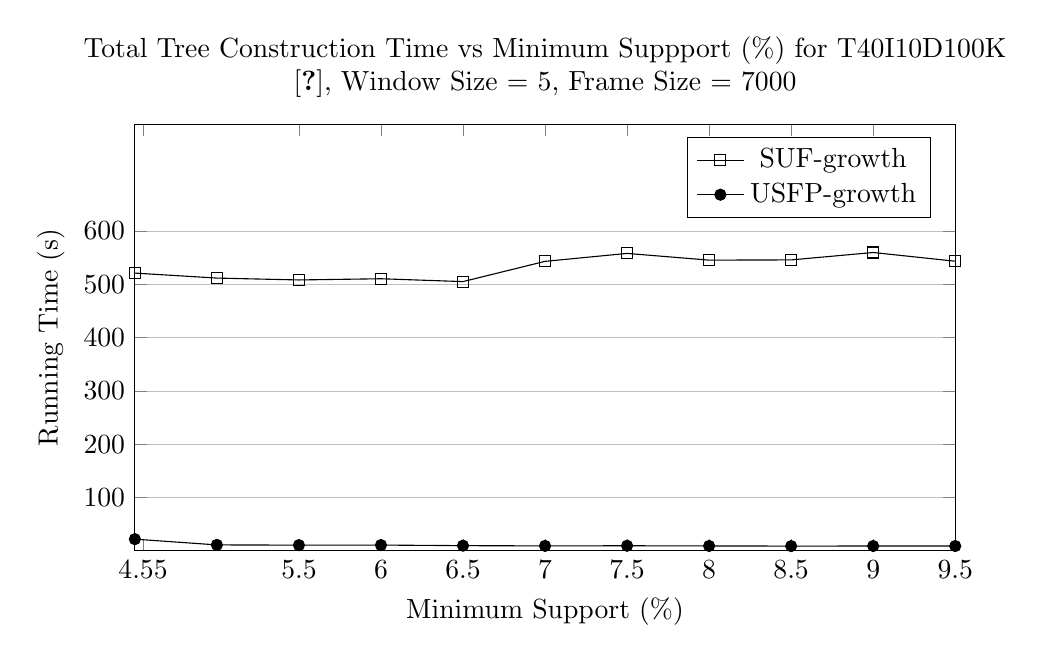
\begin{tikzpicture}
	\begin{axis}[
	title={\parbox{\linewidth}{\centering Total Tree Construction Time vs Minimum Suppport (\%) for T40I10D100K ~\cite{dataset}, Window Size = 5, Frame Size = 7000}},
	width=12cm,
	height=7cm,
    xlabel={Minimum Support (\%) },
    ylabel={Running Time (s)},
    xmin=4.5, xmax=9.5,
    ymin=0, ymax=800,
    xtick={4.55,5.5,6,6.5,7,7.5,8,8.5,9,9.5},
    ytick={100,200,300,400,500,600},
    legend pos=north east,
    ymajorgrids=true,
    grid style={line width=.2pt,draw=gray!50},
]
 
\addplot[
    solid, every mark/.append style={solid, fill=gray}, mark=square
    ]
    coordinates {
			(4.5,520.723)
			(5  ,511.365)
			(5.5,507.854)
			(6  ,510.12 )
			(6.5,504.767)
			(7  ,542.742)
			(7.5,557.633)
			(8  ,545.039)
			(8.5,545.444)
			(9  ,559.335)
			(9.5,542.996)

	};
    \addlegendentry{SUF-growth}
\addplot[
    solid, every mark/.append style={solid, fill=black}, mark=*
    ]
    coordinates {
		(4.5,21.814)
		(5  ,11.035)
		(5.5,10.601)
		(6  ,10.723)
		(6.5,9.646 )
		(7  ,9.177 )
		(7.5,9.427 )
		(8  ,9.092 )
		(8.5,8.8   )
		(9  ,8.95  )
		(9.5,8.883 )

};
    \addlegendentry{USFP-growth}
 
\end{axis}
\end{tikzpicture}
%\end{document}
%%%mark = star, diamond, square, otimes
%\documentclass{article}
%\usepackage{pgfplots}
%\usepackage[justification=centering]{caption}
%\pgfplotsset{compat=newest}
%\begin{document}
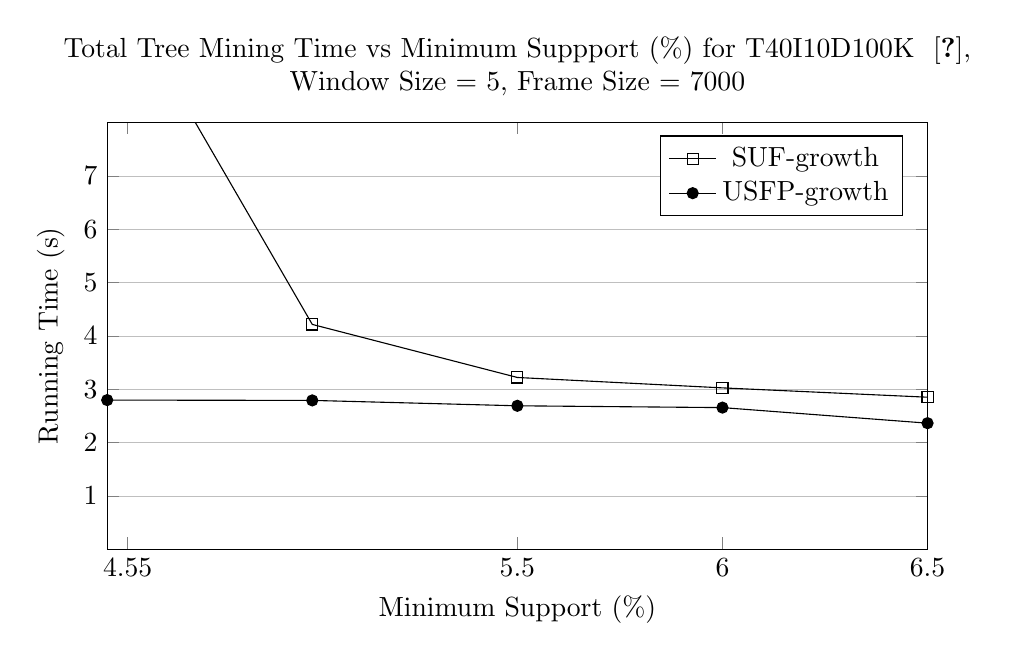
\begin{tikzpicture}
\begin{axis}[
	title={\parbox{\linewidth}{\centering Total Tree Mining Time vs Minimum Suppport (\%) for T40I10D100K ~\cite{dataset}, Window Size = 5, Frame Size = 7000}},
	width=12cm,
	height=7cm,
    xlabel={Minimum Support (\%) },
    ylabel={Running Time (s)},
    xmin=4.5, xmax=6.5,
    ymin=0, ymax=8,
    xtick={4.55,5.5,6,6.5},
    ytick={1,2,3,4,5,6,7},
    legend pos=north east,
    ymajorgrids=true,
    grid style={line width=.2pt,draw=gray!50},
]
 
\addplot[
    solid, every mark/.append style={solid, fill=gray}, mark=square
    ]
    coordinates {
			(4.5,10.856)
			(5  ,4.216 )
			(5.5,3.221 )
			(6  ,3.026 )
			(6.5,2.851 )


};
    \addlegendentry{SUF-growth}
\addplot[
    solid, every mark/.append style={solid, fill=black}, mark=*
    ]
    coordinates {
			(4.5,  2.797)
			(5  , 2.791)
			(5.5,2.69 )
			(6  ,2.656 )
			(6.5,2.364 )


};
    \addlegendentry{USFP-growth}
 
\end{axis}
\end{tikzpicture}
%\end{document}
%%%mark = star, diamond, square, otimes
%\documentclass{article}
%\usepackage{pgfplots}
%\usepackage[justification=centering]{caption}
%\pgfplotsset{compat=newest}
%\begin{document}
\begin{figure}[!h]
\centering

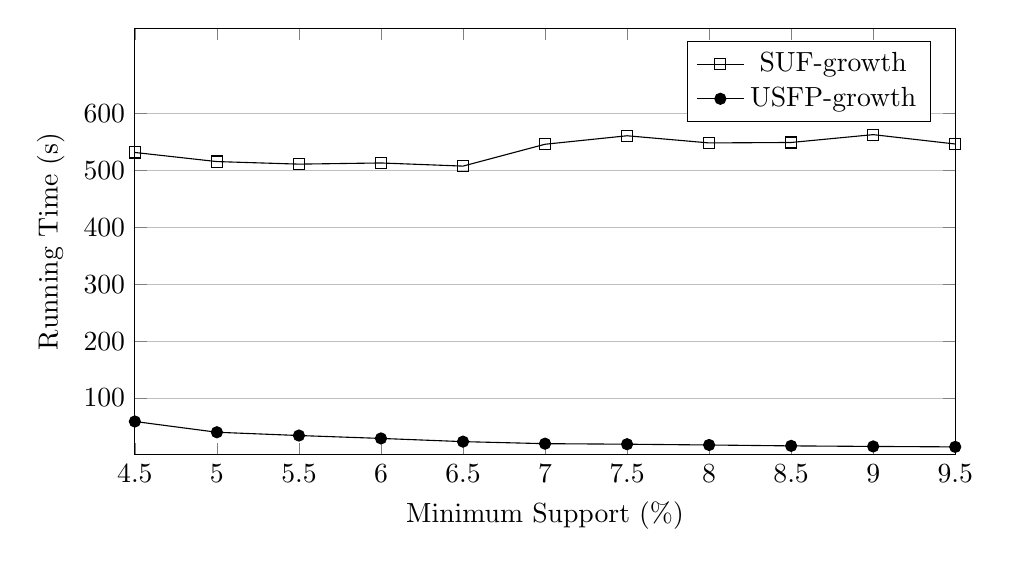
\begin{tikzpicture}
\begin{axis}[
 width=12cm,
   height=7cm,
    xlabel={Minimum Support (\%) },
    ylabel={Running Time (s)},
    xmin=4.5, xmax=9.5,
    ymin=0, ymax=750,
    xtick={4.5,5,5.5,6,6.5,7,7.5,8,8.5,9,9.5},
    ytick={100,200,300,400,500,600},
    legend pos=north east,
    ymajorgrids=true,
    grid style={line width=.2pt,draw=gray!50},
]
 
\addplot[
    solid, every mark/.append style={solid, fill=gray}, mark=square
    ]
    coordinates {
			(4.5,531.579)
			(5  ,515.581)
			(5.5,511.075)
			(6  ,513.146)
			(6.5,507.618)
			(7  ,546.032)
			(7.5,560.952)
			(8  ,548.354)
			(8.5,549.139)
			(9  ,562.928)
			(9.5,546.47 )

};
    \addlegendentry{SUF-growth}
\addplot[
    solid, every mark/.append style={solid, fill=black}, mark=*
    ]
    coordinates {
			(4.5,58.652)
			(5  ,39.735)
			(5.5,33.993)
			(6  ,28.892)
			(6.5,23.262)
			(7  ,19.669)
			(7.5,18.735)
			(8  ,17.355)
			(8.5,15.785)
			(9  ,14.803)
			(9.5,14.013)

};
    \addlegendentry{USFP-growth}
 
\end{axis}
\end{tikzpicture}
\caption{Total Time (Tree Construction + Mining + False Positive Reduction) vs Minimum Suppport (\%) \\(Window Size = 5, Frame Size = 7000) for T40I10D100K database}
\label{result:t10_total}
\end{figure}
%\end{document}
\subsection{Memory Comparison}
%mark = star, diamond, square, otimes
%\documentclass{article}
%\usepackage{pgfplots}
%\usepackage[justification=centering]{caption}
%\pgfplotsset{compat=newest}
%\begin{document}
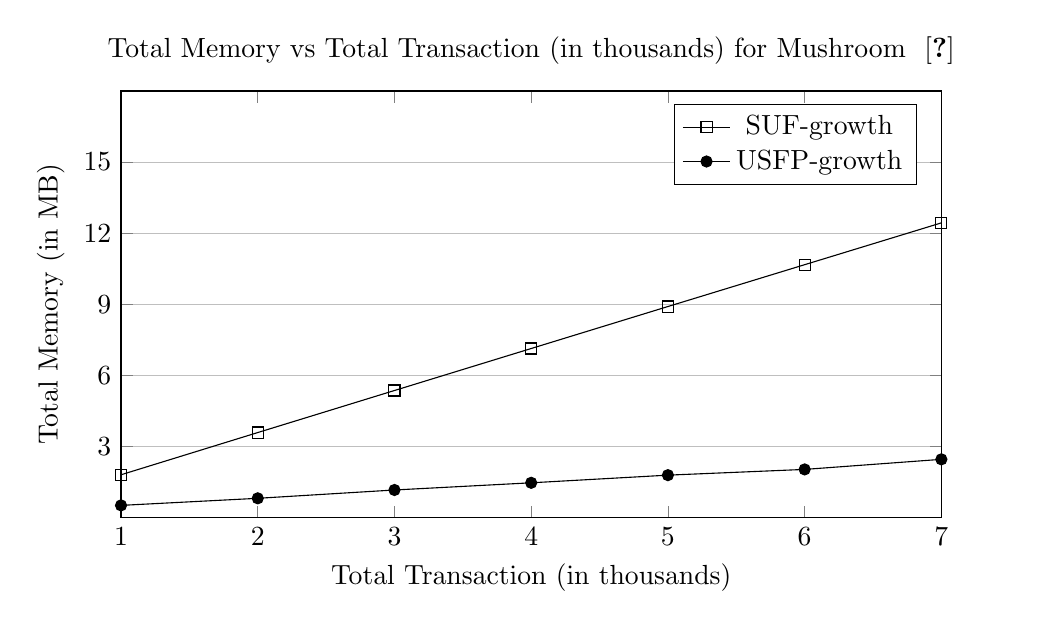
\begin{tikzpicture}
\begin{axis}[
	title={\parbox{\linewidth}{\centering Total Memory vs Total Transaction (in thousands) for Mushroom ~\cite{dataset}}},
	width=12cm,
	height=7cm,
    xlabel={Total Transaction (in thousands) },
    ylabel={Total Memory (in MB) },
    xmin=1, xmax=7,
    ymin=0, ymax=18,
    xtick={1,2,3,4,5,6,7},
    ytick={3,6,9,12,15},
    legend pos=north east,
    ymajorgrids=true,
    grid style={line width=.2pt,draw=gray!50},
]
 
\addplot[
    solid, every mark/.append style={solid, fill=gray}, mark=square
    ]
    coordinates {
			(1,1.807  )
			(2,3.588  )
			(3,5.362  )
			(4,7.134     )
			(5,8.905  )
			(6,10.670 )
			(7,12.434  )



	};
    \addlegendentry{SUF-growth}
\addplot[
    solid, every mark/.append style={solid, fill=black}, mark=*
    ]
    coordinates {
			(1,.5152  )
			(2,.814  )
			(3,1.165 )
			(4,1.468 )
			(5,1.791  )
			(6,2.033 )
			(7,2.458 )


};
    \addlegendentry{USFP-growth}
 
\end{axis}
\end{tikzpicture}
%\end{document}
%%%mark = star, diamond, square, otimes
%\documentclass{article}
%\usepackage{pgfplots}
%\usepackage[justification=centering]{caption}
%\pgfplotsset{compat=newest}
%\begin{document}
\begin{figure}
\centering

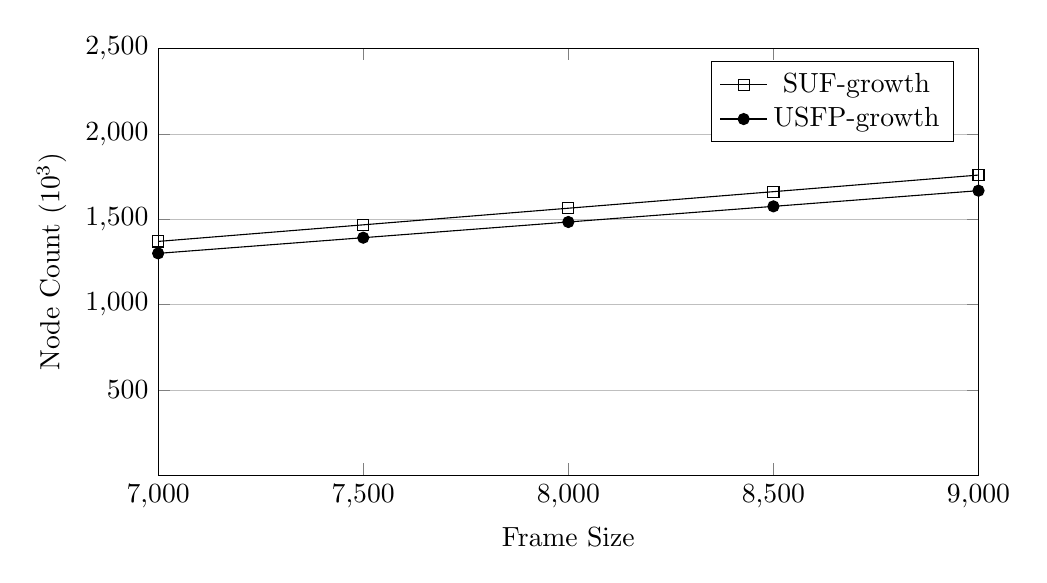
\begin{tikzpicture}
\begin{axis}[
 width=12cm,
   height=7cm,
    xlabel={Frame Size },
    ylabel={Node Count ($10^3$)},
    xmin=7000, xmax=9000,
    ymin=0, ymax=2500,
    xtick={7000,7500,8000,8500,9000},
    ytick={500,1000,1500,2000,2500},
    legend pos=north east,
    ymajorgrids=true,
    grid style={line width=.2pt,draw=gray!50},
]
 
\addplot[
    solid, every mark/.append style={solid, fill=gray}, mark=square
    ]
    coordinates {
			(7000,1369.555 )
			(7500,1466.766 )
			(8000,1564.122 )
			(8500,1661.100 )
			(9000,1758.412 )
			(9500,1855.734 )

	};
    \addlegendentry{SUF-growth}
\addplot[
    solid, every mark/.append style={solid, fill=black}, mark=*
    ]
    coordinates {
					(7000,1299.510)
		(7500,1391.388)
		(8000,1483.378)
		(8500,1574.984)
		(9000,1666.912)
		(9500,1758.773)

};
    \addlegendentry{USFP-growth}
 
\end{axis}
\end{tikzpicture}
\caption{Total Tree Node vs Frame Size (Window Size = 5) for T40I10D100K database}
\label{result:t10_total_mem_node}
\end{figure}
%\end{document}
%
%\end{document}